\section{Imaging artifacts}
\label{sec:imaging}

Noise in tomography is unavoidable, and it makes segmentation harder because it
further obscures the boundaries between materials.  Materials may be well
separated at some angles but overlap at other in the resulting projections.
The effects are manifested in the 3D-reconstruction as numerical shifts in
voxel values as a function of their position. This is a direct result of a
misrepresented attenuation along the axis of the incoming X-rays.  The
dependency on orientation illustrates how voxel intensity values are not
globally fixed. Instead, how a certain material is represented in intensity is
highly dependent on its position relative to neighboring regions. The same
material with the same density can thus be represented as multiple intensities
within the same sample.  Some noise can thus be uniformly distributed across
images, such as that removed by flat-field correction, while other noise is
very spatially dependent on its surrounding regions. By knowing the composition
and positioning of the materials being imaged, we can correct some of these
effects during segmentation.

We will refer to noise as voxels being numerically altered to obscure features
in the image, whereas artifacts are regarded as regions that falsely appear to
contain notable features.

\begin{figure}
  \centering
  \begin{tabular}{cc}
    \!\!\!\!\!\!(a)\!\!\!&\begin{tabular}{c}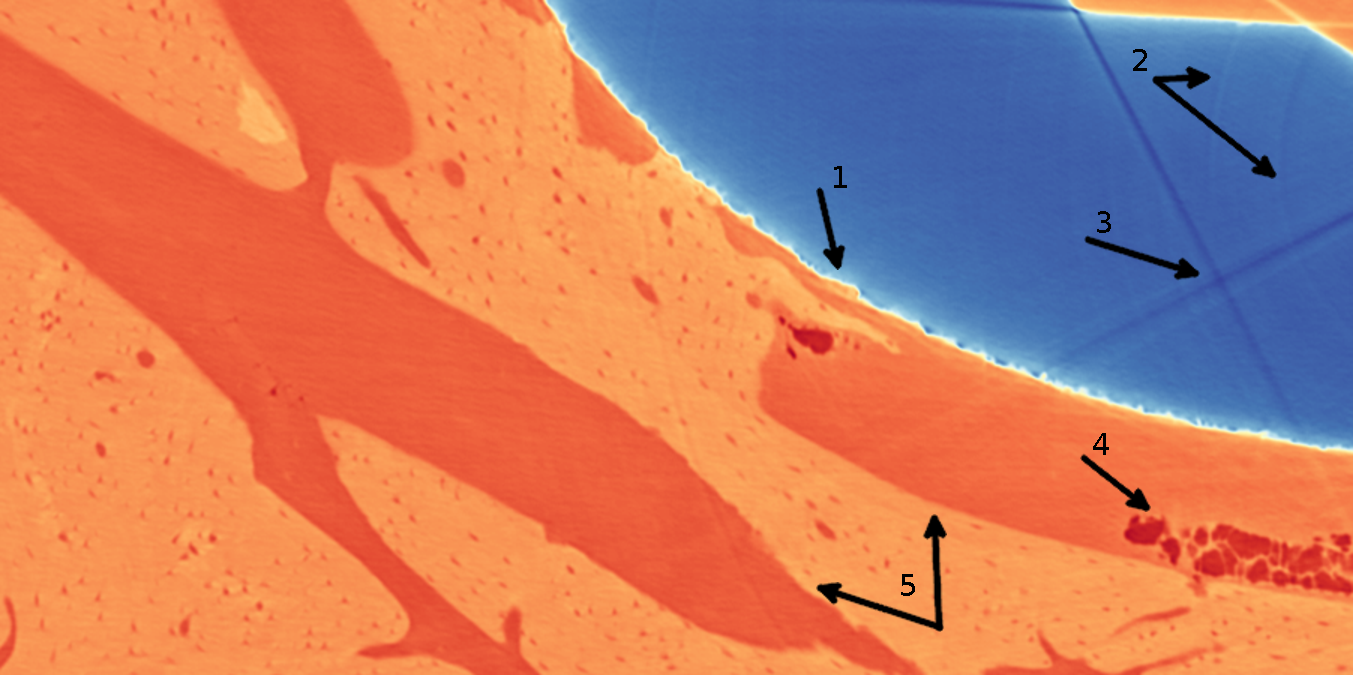
\includegraphics[width=0.85\columnwidth]{figures/770c_pag_segmented_yx_raw_annotated.pdf}\end{tabular}\\
    \!\!\!\!\!\!(b)\!\!\!&\begin{tabular}{c}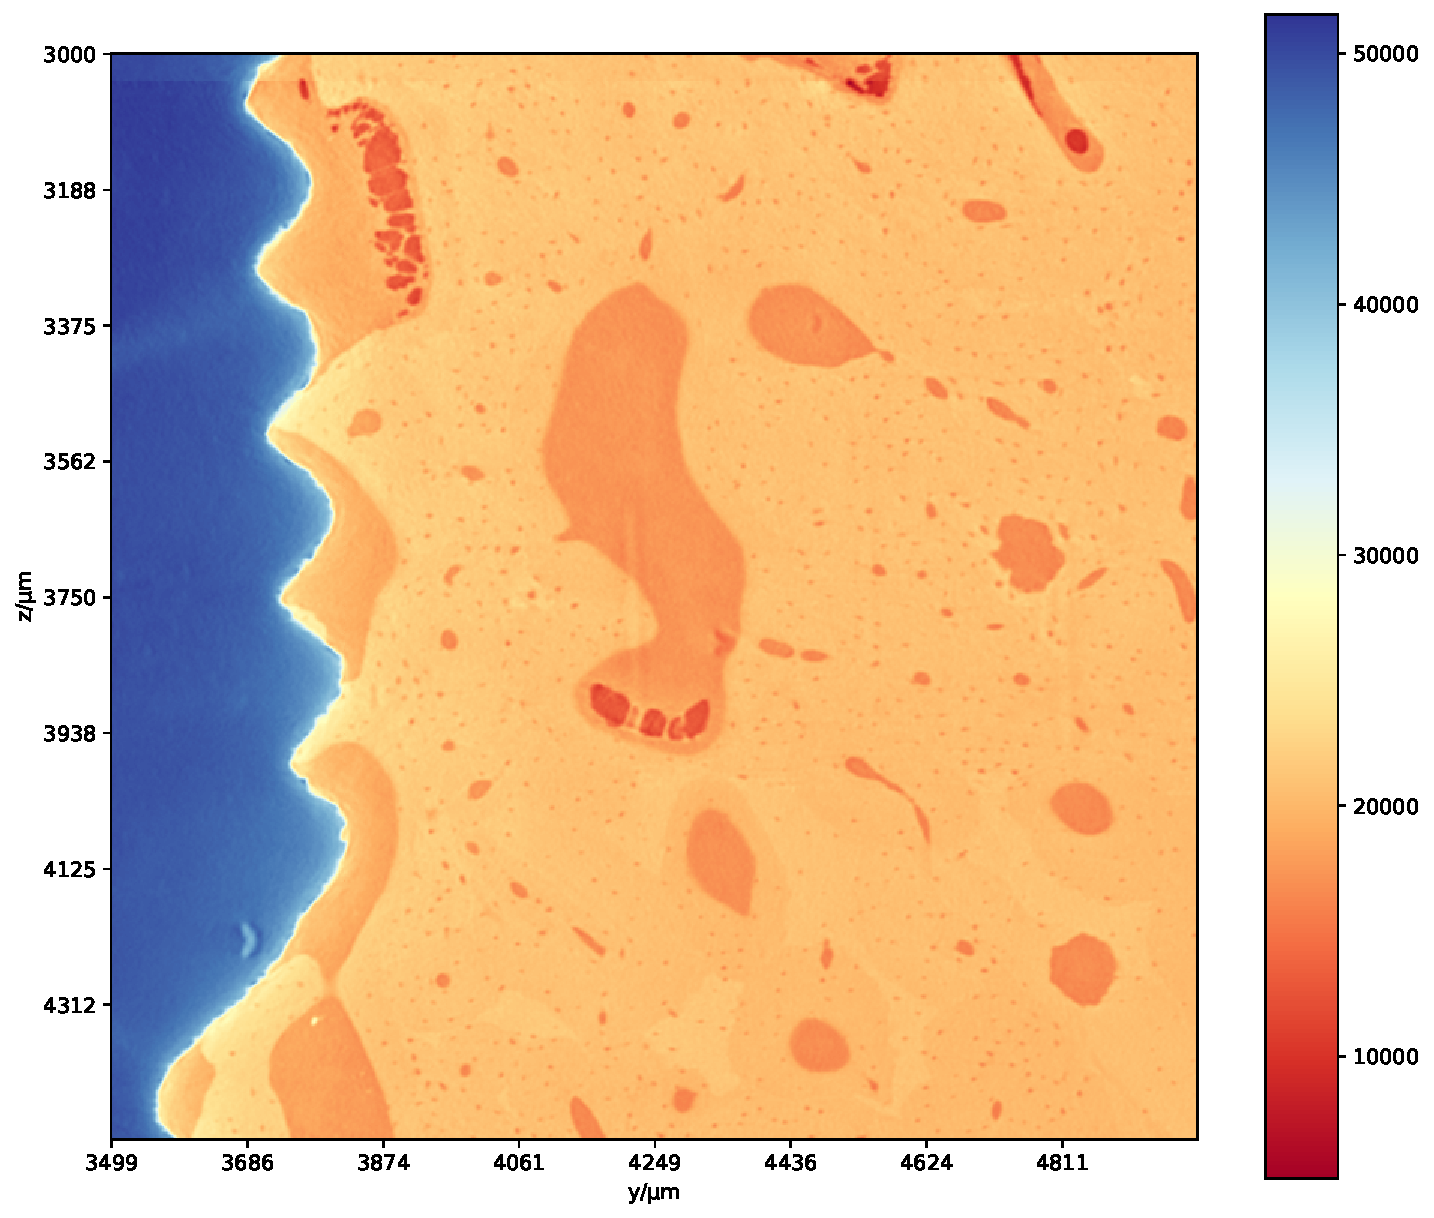
\includegraphics[width=0.85\columnwidth]{generated/770c_pag_roi_zy.pdf}\end{tabular}\\
  \end{tabular}
  \caption{
    (a) Region of size 1 mm $\times$ 2 mm within a slice in the YX-plane.
    (a.1) Implant glow, metal artifacts
    (a.2) Ring artifacts, also notice multiple concentric rings
    (a.3) Streaks, which are seen to continue through the full 2d-slice
    (a.4) Air bubbles in the resin-filled blood vessels
    (a.5) Contrast-shifted glow, in upper vs lower blood vessel, displaying
	  different numerical values in same resin
    (b) Region of size 1.5 mm $\times$ 1.5 mm within a slice in the ZY-plane
	around the
    smaller threaded part of the titanium implant.
  }
\label{fig:slices}
\end{figure}

In \Cref{fig:slices}, we see zoomed-in regions of the YX- and ZY-planes of the
same sample as shown in \Cref{fig:3viewsample}.  Our visual systems
automatically correct for most of the distortions. However, at various
distances from the implant, blood vessel voxels have higher values than bone
voxels further out. As we approach the implant, the value shifts accelerate and
become highly non-linear.  Both planes display a broad selection of the various
types of noise sources found in the data.

We will only cover the most dominant phenomena that result in noise and
artifacts affecting the reconstructed image. Many other sources will likewise
contribute noise and artifacts, but a full study is beyond the scope of this
work and can be found in existing
literature~̣\citep{noise_and_artifacts_1,noise_and_artifacts_2}. The numbers in
parentheses refer to corresponding arrows in \Cref{fig:slices} that illustrate
how the mentioned phenomena are manifested in the data. Note that not all
effects have a corresponding arrow.

% most pronounced effects are: streaks, glow, ring artifacts
\begin{itemize}
	\item \textbf{Erroneous volumes (4):} During sample preparation, the
		resin has not successfully filled out all crevices in the blood
		vessels. Instead, some air pockets are left within the resin,
		changing the effective density and thereby absorption. This is
		an effect which we cannot correct, because it is in fact
		present in our data. It appears in the tomographic slices
		\Cref{fig:slices} as dark spots in the otherwise lighter resin. 
	\item \textbf{Dark and bright streaks (3):} Streaking artifacts occur
		close to regions with very high absorption, such as metal
		implants, but also to some degree in the transition from dense
		bone to softer tissue.  This effect is also called photon
		starvation, due to the lowered amount of photons reaching the
		detector through more hardened trajectories due to higher
		absorption \citep{srnoise}. Scattering around high density
		regions also makes up a significant contribution, adding to the
		streaking artifacts \citep{scatter_sr_ct}.
	\item \textbf{Cupping effect:} A commonly occurring artifact occurs
		when beams pass homogeneous cylindrical objects. Since beams
		passing the middle will have to traverse more material compared
		to the edges, the beam is hardened more towards the center and
		intensity becomes lower as a result. This can manifest itself
		in what erroneously looks to be dense peripheral regions at the
		edges. A cupping effect also arises from scattering which leads
		to a reduction in low contrast sensitivity
		\citep{srnoise}.
	\item \textbf{Phase contrast (1,5):} Phase contrast is used to enhance
		the contrast around soft tissue where the contrast from pure
		absorption is insufficient \citep{phasecontrast}. It can
		however also induce noise, such as fringes around the edges
		between different materials within the sample\citep{srnoise}.
		Similar to the dark and bright streaks artifacts, these effects
		show up as misrepresentations of the voxel values. This is
		especially prominent at the transitional edges between
		biological tissue and bone \citep{srnoise}.
	\item \textbf{Ring artifacts (2):} Looking at the XY-plane in
		\Cref{fig:slices}(a) we see clear concentric ring artifacts
		emanating from the center of the sample, and at strong edges of
		the titanium implant. It propagates strongly through the large
		region of air behind the implant. This effect arises from
		imperfections in the scanner setup and is typically come from
		uncalibrated or defect adjacent detector elements. For
		synchrotron radiation sources it can also occur from shifts and
		vibrations in the monochromator crystal \citep{ringartefacts}.
	\item \textbf{Scattering:} Lower energy rays mostly contribute noise
		from scattering effects. A ray will propagate through a
		material, get scattered and diffract from its initial
		trajectory. This gives a misrepresentation of the attenuation
		along its initial trajectory. The artifacts seen from
		scattering are similar in nature to those formed by beam
		hardening, due to how both phenomena effectively misrepresent
		the measured attenuation.  For X-ray energy levels used for the
		data presented here, of 50 keV and above, Compton scattering is
		the dominant type.  Coherent scattering is not very dominating
		at 50 keV, but incoherent scattering slightly dominates for
		Titanium at 50 keV. Incoherent Compton scattering will add an
		overall haze and reduce contrast in the image
		\citep{Compton}\citep{xray-attenuation-10-kev-100-mev}\citep{attenuation-cross-sections}.
\end{itemize}

\begin{figure}
    \centering
    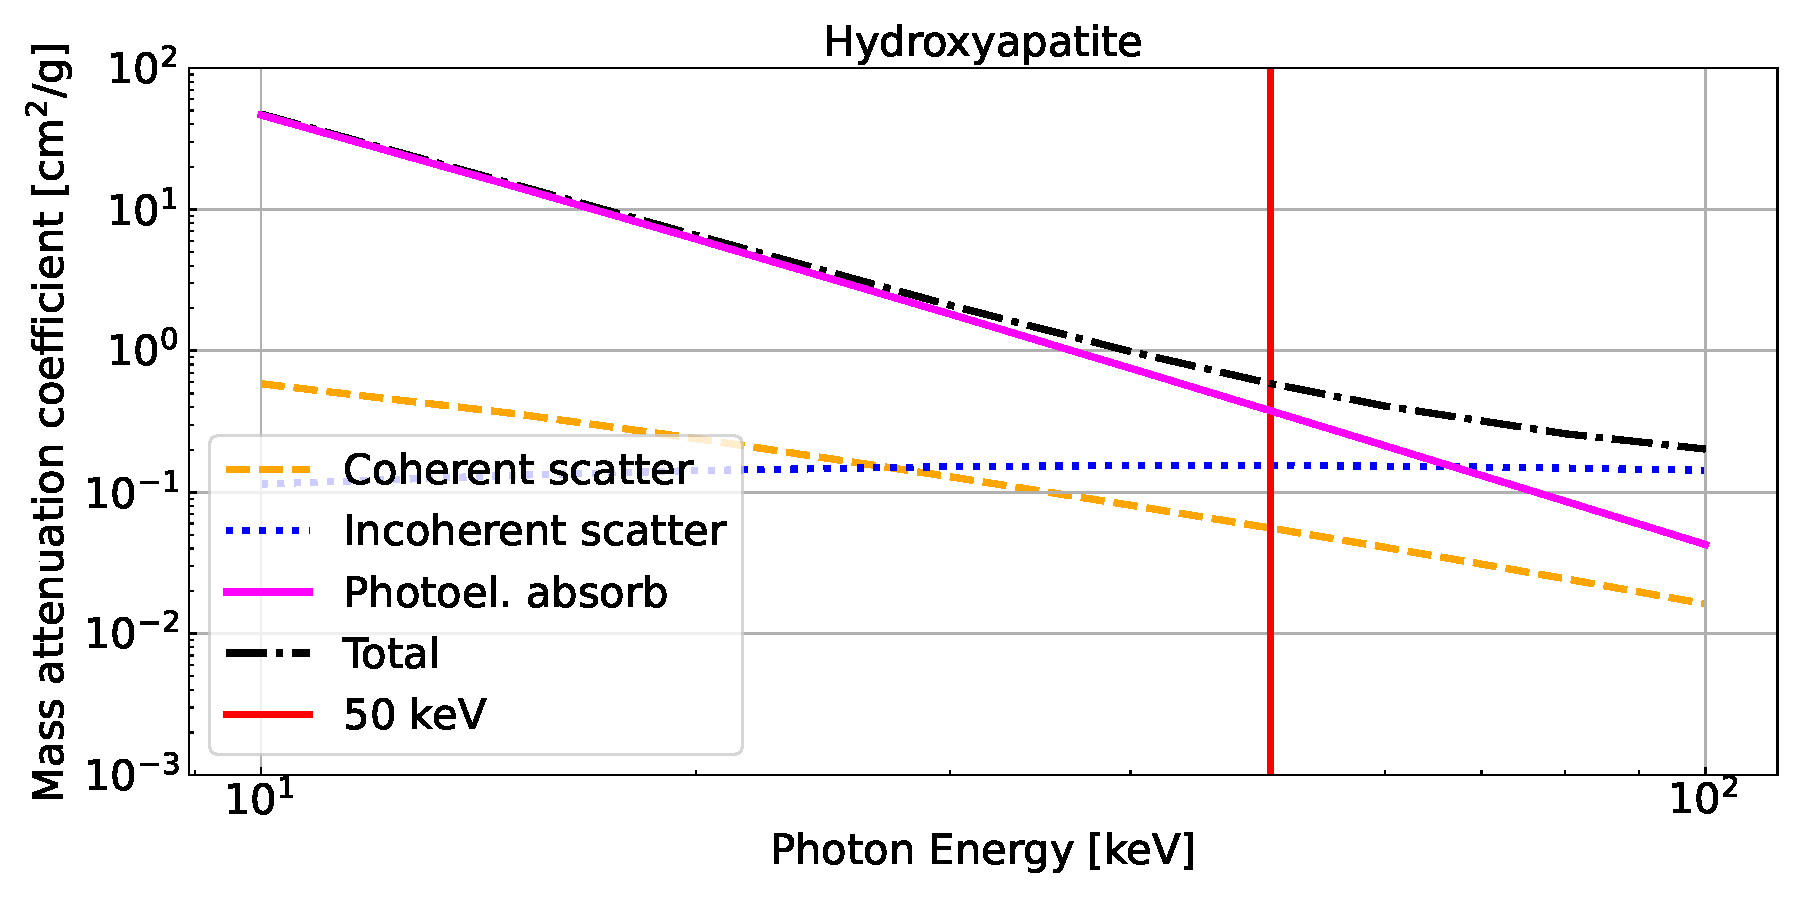
\includegraphics[width=\linewidth]{figures/attenuation_bone.pdf}
    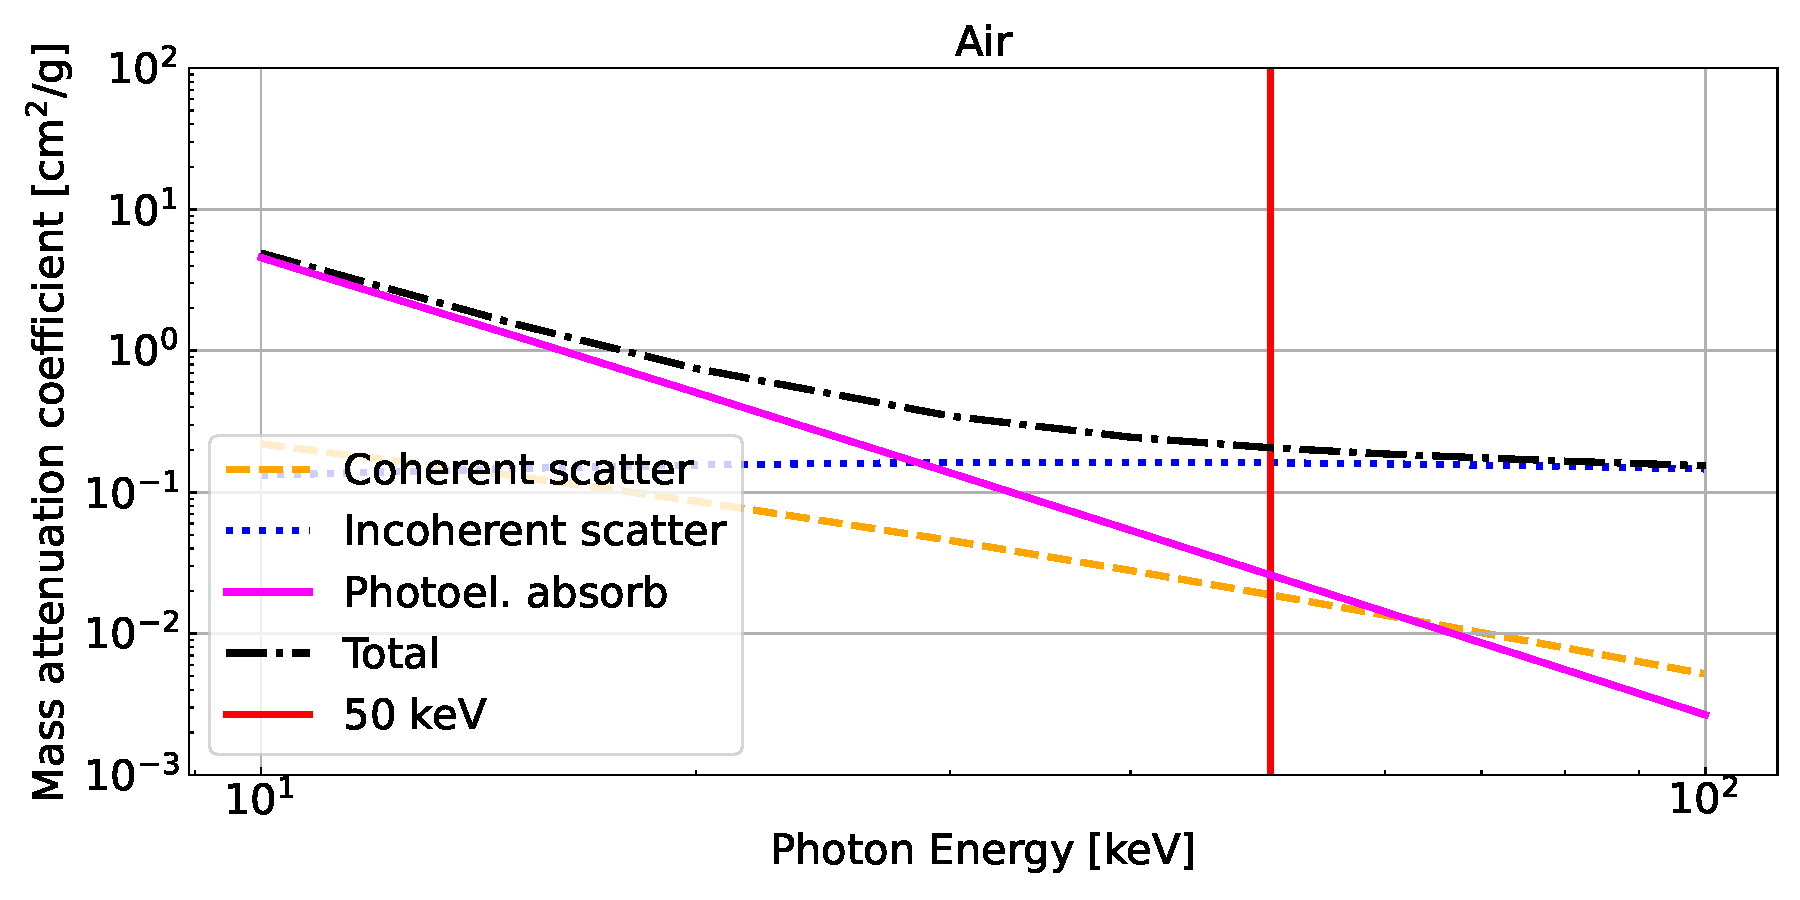
\includegraphics[width=\linewidth]{figures/attenuation_air.pdf}
    \caption{
	    % TODO (James): Mangler måske et par ord (kontekst) omkring hvorfor vi snakker om Hydroxyapatite ift knogler?
	    Mass attenuation coefficients for Ca$_{5}$(PO$_{4}$)$_{3}$(OH)
	    (Hydroxyapatite) and air, using a mixture (78\% N$_{2}$, 21\% O, 1\%
	    Ar). The vertical line marks 50 keV at which our data was acquired. The
	    mass attenuation coefficients are computed using NIST XCOM
	    \citep{NIST-XCOM}.
    }
\label{fig:attenuation}
\end{figure}

The absorption coefficient becomes larger with increasing density and atomic
number of the absorbing material. Conversely, the effective absorption is
decreased for increasing energy of the incoming X-ray beam.
\Cref{fig:attenuation} shows the dominating photon interactions and the
contribution to attenuation over the relevant range of energies. Relative to
Hydroxyapatite, the mass attenuation coefficients for blood and air is
essentially the same. The figure shows that incoherent scattering (Compton
scattering) is the prevalent interaction for air, blood and water, with slightly
smaller contribution from coherent scattering (Rayleigh, Thompson) and
photoelectric absorption. For Hydroxyapatite, photoelectric absorption is about
an order of magnitude more significant, exceeding the contribution of incoherent
and coherent scattering. This intuitively makes sense since Hydroxyapatite has a
higher effective atomic number $Z_{bone}$~16~\cite{hydroxyapatite_absorption},
compared to blood $Z_{blood}$~6~\cite{effective_atomic_number}.

%%% Local Variables:
%%% mode: latex
%%% TeX-master: "main"
%%% End: